% !TEX encoding = IsoLatin
% Modificado: 2017 nov 18 - 02:33
\documentclass[svgnames]{beamer}
%\documentclass[svgnames,handout]{beamer}
% --------------------------------------------------------------------------
%\usepackage[latin1]{inputenc}
\usepackage[spanish]{babel}
\usepackage[T1]{fontenc}
\usepackage{amsmath,amssymb}
\usepackage{bm}
\usepackage{multimedia}
\usepackage{cancel}
%\usepackage{jgn}
% --------------------------------------------------------------------------
%\usepackage{graphicx}
%\usepackage{enumitem}
%\usepackage{hyperref}
%\hypersetup{%
%    pdftitle={máster IECM 2009-10 - MEF - Vigas},
%    pdfkeywords = {Elementos Finitos, Mecánica Computacional},
%    pdfauthor = {Jose M.ª Goicolea},
%    pdfpagemode = UseNone,
%    % menucolor=cyan,
%    % colorlinks=true,
%    %baseurl = {file:/home/goico/demos/},
%    %pdfpagemode = {FullScreen}
%}%
%..............................................................................
\newcommand{\trebol}{\textcolor{SpringGreen}{$\clubsuit$}\ }
\newcommand{\pica}{\textcolor{blue}{$\spadesuit$}\ }
\newcommand{\carreau}{\textcolor{magenta}{$\diamondsuit$}\ }
\newcommand{\corazon}{\textcolor{red}{$\heartsuit$}\ }
\newcommand{\bul}{$\bullet$\ }
\newcommand{\mcolorbox}[1]{\fcolorbox{black}{PeachPuff}{\ensuremath{{#1}}}} 
\newcommand{\tcolorbox}[1]{\fcolorbox{black}{PeachPuff}{{#1}}} 
\newcommand{\blue}[1]{\textcolor{blue}{#1}}
\newcommand{\red}[1]{\textcolor{red}{#1}}
\newcommand{\Green}[1]{\textcolor{Green}{#1}}
\let\club=\trebol
\let\diamante=\carreau
\let\heart=\corazon
\let\spade=\pica
% --------------------------------------------------------------------------
\DeclareMathSymbol{\dr}{\mathalpha}{operators}{`d}
\DeclareMathSymbol{\e}{\mathalpha}{operators}{`e}
\def\eqdef{\buildrel\text{def}\over =}
\DeclareMathOperator{\tr}{tr}
% --------------------------------------------------------------------------
%------------------------------------------------------------------------------
%\usetheme{default}
\usetheme{Frankfurt}
\usecolortheme{seahorse}
\usecolortheme{rose}
\useinnertheme{circles}
\useoutertheme{infolines}
\setbeamertemplate{headline}{}
\setbeamertemplate{footline}{%
  \leavevmode%
  \hbox{%
  \begin{beamercolorbox}[wd=.3\paperwidth,ht=2.25ex,dp=1ex,center]{author in head/foot}%
    \usebeamerfont{author in head/foot}\insertshortauthor{} -- \insertshorttitle
  \end{beamercolorbox}%
  \begin{beamercolorbox}[wd=.48\paperwidth,ht=2.25ex,dp=1ex,center]{title in head/foot}%
    \usebeamerfont{title in head/foot}\insertsection{} -- \insertsubsection
  \end{beamercolorbox}%
  \begin{beamercolorbox}[wd=.22\paperwidth,ht=2.25ex,dp=1ex,right]{date in head/foot}%
    \usebeamerfont{date in head/foot}\insertshortdate{}\hspace*{1em}
    \insertframenumber{} / \inserttotalframenumber\hspace*{2em} 
  \end{beamercolorbox}}%
  \vskip0pt%
}

\setbeamertemplate{navigation symbols}{\vbox{%
  \only<beamer| handout:0>{\hbox to 7mm{\insertslidenavigationsymbol}}%
  \hbox to 7mm{\insertframenavigationsymbol}}}
%\setbeamertemplate{navigation symbols}[only frame symbol]
\usebeamertemplate{logo}
\setbeamertemplate{itemize item}[ball]
\setbeamertemplate{section in toc}[ball]
%\setbeamertemplate{subsection in toc}[ball]
\usefonttheme{structurebold}
\usefonttheme[onlymath]{serif}
\setbeamercovered{dynamic}
\setbeamertemplate{blocks}[rounded][shadow=true]
%\setbeamertemplate{itemize item}{\protect\pica}
%\setbeamertemplate{itemize subitem}{\protect\carreau}
%------------------------------------------------------------------------------

\title[Beam FE]{Structural Models: Beam Elements}
\subtitle{Finite Element Methods}
%\title[Vigas]{Modelos Estructurales: Vigas}
%\subtitle{Método de los Elementos Finitos}
%\author[J.M. Goicolea (UPM)]{José M. Goicolea}
\institute[UPM]{
  \emph{
  %Grupo de Mecánica Computacional,
  %Computational Mechanics Group, %\\
  %Escuela de Ingenieros de Caminos,\\
  %Universidad Politécnica de Madrid%
}}
\titlegraphic{
  
\includegraphics[height=15mm]{000logos/upm}
  \hfill
  \includegraphics[height=15mm]{000logos/logo14c}
  \hfill
  
\includegraphics[height=15mm]{000logos/caminos}}

\date[19.10.2023]{19 October 2023}
%\date[24.11.2022]{24 November 2022}
%\date[25.11.2021]{25 November 2021}
%\date[26.11.2020]{26 November 2020}


\begin{document}

\logo{}     % En la página del título no queremos logo, ya hay escudos
\begin{frame}[plain]
  \titlepage
\end{frame}

% en las páginas siguientes aparecerá este logo
\logo{\vbox{%
    \hbox to 6mm{
\includegraphics[width=6mm]{000logos/upm}}%
%    \vskip 1mm%
%    \hbox to 7mm{\includegraphics[width=7mm]{000logos/logo14c}}%
}}

\begin{frame}[plain]
%\frametitle{Índice}
\frametitle{Outline}
\tableofcontents%,pausesections]
\end{frame}

\section{Introduction}
%\AtBeginSection[]
%{
%  \begin{frame}[plain]
%%    \frametitle{Índice}
%    \frametitle{Outline}
%    \tableofcontents[currentsection,currentsubsection]
%  \end{frame}
%}
\AtBeginSubsection[]
{
  \begin{frame}<beamer|handout>[plain]
    \frametitle{Índice}
    \tableofcontents[currentsection,currentsubsection]
  \end{frame}
}

\subsection{Motivation}

\begin{frame}
\frametitle{Las Piedras. L=19$\times$63.5=1206.5 m; H=92 m}
\framesubtitle{Córdoba--Málaga HS line}
 \centering
 \includegraphics[width=0.95\linewidth]{puentes_fotos_piedras/img_0557rr}\par 
% \enf{Viaduct ``Las Piedras''. Córdoba--Málaga}\\
% Length $19\times 63.5 = 1206.5$ m; $92$ m pier\par
\end{frame}

\begin{frame}
\frametitle{Contreras viaducts; Arch L=261 m}
\framesubtitle{Madrid--Valencia HS line}
%\frametitle{Contreras; Arco L=261 m.}
 \centering
 \includegraphics[width=0.9\textwidth]{madrid2011-torroja_pres_nhsrb/contreras-2}
 \par
% \\
% \centering\bf\tbluePas{%
%Viaducto sobre el embalse de Contreras. Madrid--Valencia.
% }\par
% \enf{%
%Contreras viaducts; Arch $L=261$ m. Madrid--Valencia.
% }\par
\end{frame}

\begin{frame}<all:0>
\frametitle{River Ulla. L=168 m, H=115 m}
\framesubtitle{Orense--Santiago HS line}
%\frametitle{Río Ulla. L=168 m, H=115 m}
 \centering
 \includegraphics[width=0.95\textwidth]{puentes_Ulla/Ulla-GilPan-cut}\par
% \enf{Viaduct on Ulla. Orense--Santiago. $L=168$ m, $H=115$ m}\paragraph{?}

\end{frame}

\begin{frame}
\frametitle{La Marota. L=381 m; Córdoba--Málaga HS line}
 \centering
 \includegraphics[width=0.50\textwidth]{LaMarota/20211021_121843-clip.jpg}\par
 \includegraphics[width=1.00\textwidth]{LaMarota/Alzado.pdf}
\end{frame}

\begin{frame}
\frametitle{Villanueva del Jalón Bridge}
\framesubtitle{Madrid-Barcelona HS line}
\begin{center}
 \includegraphics[height=2.7cm]{jalon-presentacion/figs/jalon.jpg}
% \includegraphics[height=2.7cm]{joliva1/figuras/vista.pdf}
 \includegraphics[height=2.7cm]{joliva1/figuras/alzado_planta_jalon.png}
\end{center}
\begin{columns}
\begin{column}{0.6\textwidth}
\begin{itemize}
\item Madrid-Barcelona High Speed Railway
\item Prestressed concrete
\item Total length: 250 m 
\item 6 spans (35 + 4 x 45 + 35)
\end{itemize}
\end{column}
\begin{column}{0.4\textwidth}
 \includegraphics[width=\linewidth]{jalon-presentacion/figs/secc_jalon.pdf}
\end{column}
\end{columns}
\end{frame}

\begin{frame}
\frametitle{Villanueva del Jalón: types of FE models}
\begin{columns}
\begin{column}{0.5\textwidth}
\centering
 \emph{Continuum} elements\\
\includegraphics[width=1.0\linewidth]{jalon-modelos/jalon-solido-g}\\
 \emph{Shell} elements\\
\includegraphics[width=1.0\linewidth]{jalon-modelos/jalon-lamina-g}
\end{column}
\begin{column}{0.5\textwidth}
\centering
 \emph{Beam} elements (ornate)
\includegraphics[width=1.0\linewidth]{jalon-modelos/jalon-vigas-render}\\
 \emph{Beam} elements (plain)
\includegraphics[width=1.0\linewidth]{jalon-modelos/jalon-vigas}
\end{column}
\end{columns}
\end{frame}

\begin{frame}
\frametitle{Villanueva del Jalón: Numerical models}
\begin{columns}
\begin{column}[]{0.5\textwidth}
\begin{center}
\includegraphics[width=1.0\textwidth]{joliva1/figuras/beams.png}\\
FEM (Beams)
\end{center}
\end{column}
\begin{column}[]{0.5\textwidth}
\begin{center}
\includegraphics[width=1.0\textwidth]{joliva1/figuras/shells.png}\\
FEM (Shells)
\end{center}
\end{column}
\end{columns}
\vspace{0.3cm}
%-----------------------------TABLE
\begin{center}
\begin{tabular}{lccc}  \cline{2-4}
& \multicolumn{3}{c}{Frequency [Hz]} \\   \cline{2-4}
& 1st lateral & 1st vertical & 1st torsion \\  \hline \hline
Beam elements & 0.623 & \textbf{3.228} & 3.498\\ \hline
Shell elements & \textbf{0.627} & 3.059 & \textbf{5.823} \\ \hline
 \end{tabular}
\end{center}
%-----------------------------TABLE-END
\end{frame}

\subsection{Beam General Assumptions}
%\subsection{General Assumptions for Beams; Equilibrium equations}
%\subsection{Vigas 2D: Hipótesis generales.  Equilibrio}

\begin{frame}
\frametitle{Beams: General Assumptions}
%\frametitle{Vigas: Hipótesis generales}
\begin{block}%
{Assumptions:}
%{Hipótesis:}
  \begin{itemize}[<+->]
    \item 
    Prismatic slender rod, with \alert{one dimension (longitudinal) much greater} than the other two (transverse) dimensions
%    Pieza prismática, con dimensión longitudinal mucho mayor que otras dos (transversales)
	\item
	\alert{Base curve} (\emph{``directriz''}) $\bm{r}_{0}(s)$, with $s=$ arc-length;
	\item
	Normal \alert{cross section} at each point, $\perp \bm{r}_{0}(s)$.\\
	\alert{Rigid} (plane and undeformable)
	\item 
	Local axes: $x$ tangent to base curve; $(y,z)$ transverse ( normal to $x$).
%    Eje $x$ longitudinal, $z$ transversal $\in$ plano, $y$ transversal $\perp$  plano
	\item
	2D beams: loads $(q_{x}, q_{z})$ and deflection $(u, w)$ within $xz$ plane
  \end{itemize}
\end{block}
\parbox{0.6\textwidth}{\includegraphics[scale=0.55]{figs/118curso05a}}%
\parbox{0.4\textwidth}{\reflectbox{\includegraphics[width=\linewidth]{madrid2011-torroja_pres_figures-pablo/modelos/puente3D}}}
\end{frame}

\begin{frame}
\frametitle{2D Beams: Section Resultants}
%\frametitle{Vigas: Definición de Resultantes}
\begin{columns}
\begin{column}{0.50\textwidth}
Axial resultant:
\begin{equation}
  N \eqdef\int_{t_{1}}^{t_{2}} \sigma_{xx}b(z)\,\dr z
\end{equation}
\pause
Shear resultant:
\begin{equation}
  V \eqdef\int_{t_{1}}^{t_{2}} \sigma_{xz}b(z)\,\dr z
\end{equation}
\pause
Bending moment:
\begin{equation}
  M \eqdef-\int_{t_{1}}^{t_{2}} z\sigma_{xx}b(z)\,\dr z
\end{equation}
\end{column}
\begin{column}{0.50\textwidth}
  \hfill\includegraphics[width=\linewidth]{figs/x-section}
%  \hfill\includegraphics[width=\linewidth]{figs/118curso00b}
\end{column}
\end{columns}
\end{frame}

\begin{frame}
\frametitle{2D Beams: Equilibrium equations}
%\frametitle{Vigas: Condiciones de Equilibrio}
%\noindent\parbox{0.40\textwidth}{
\begin{columns}
\begin{column}{0.40\textwidth}
Axial equilibrium
\begin{equation}
  \frac{\dr N}{\dr x}+q_x=0; \label{eq:Nq}
\end{equation}
\pause
Shear equilibrium
\begin{equation}
  \frac{\dr V}{\dr x}+q_z=0; \label{eq:Vq}
\end{equation}
\pause
Bending moment equilibrium
\begin{equation}
  \frac{\dr M}{\dr x}+V=0 \label{eq:MV}
\end{equation}
\end{column}
%}
\begin{column}{0.58\textwidth}
%\parbox{0.58\textwidth}{
  \hfill\includegraphics[scale=0.5]{figs/118curso00c}
  \hspace{1ex}
\end{column}
\end{columns}
%}
\visible<3->{\club 
Universal validity, even with material or geometric nonlinearities
%Leyes válidas en cualquier instancia (incluso no lineal).
}
\end{frame}

\section{Bernoulli--Euler Beam}
%\section{Modelo de vigas de Bernoulli--Euler}

\subsection{Strong and Weak Formulations}
%\subsection{Formulaciones fuerte y débil}

\begin{frame}
\frametitle{Bernoulli-Euler Assumptions}
%\frametitle{Hipótesis de Bernoulli-Euler}
\begin{columns}
\begin{column}{0.4\textwidth}
\begin{enumerate}
  \item 
  Prismatic rod, with base curve \emph{(``directriz'')}  $\bm{r}_{0}(s)$ (line of centroids)
%  Pieza prismática, directriz
  \newcounter{enumi_saved}
  \setcounter{enumi_saved}{\value{enumi}}
\end{enumerate}
\end{column}
\begin{column}{0.6\textwidth}
  \includegraphics[scale=0.5]{figs/118curso05a}
\end{column}
\end{columns}
\begin{columns}
\begin{column}{0.99\textwidth}
\begin{enumerate}
  \setcounter{enumi}{\value{enumi_saved}}
  \item
  After deformation, plane cross sections $(yz)$ remain plane and \alert{normal to the base curve}
%  Secciones planas normales a directriz permanecen planas y  \textcolor{red}{normales a la directriz}
  \item 
  (2D) Displacements normal to the beam ($w\eqdef u_{z}$) are uniform along the cross section and equal to those of the base curve:
%  Desplazamientos normales a la viga son uniformes sobre la sección, e iguales a los de la directriz:
  \begin{equation}
    \boxed{w(x,z)=w(x).} \label{eq:wx}
  \end{equation}
  \item 
  (2D) Plane stress:
%  Tensión plana: 
  \begin{equation}
  \boxed{\sigma_{zz}=0.}
  \end{equation}
\end{enumerate}
\end{column}
\begin{column}{0.01\textwidth}
\strut
\end{column}
\end{columns}
\end{frame}

\begin{frame}
\frametitle{Displacements (2D)}
%\frametitle{Desplazamientos}
\begin{columns}
\begin{column}{0.50\textwidth}
\includegraphics[width=\linewidth]{figs/118curso06a}
\end{column}
\begin{column}{0.50\textwidth}
\begin{itemize}
\item
Rotation of cross section:
%Giro de sección: 
$\theta$ \\
\item
Rotation of tangent to base curve:
%Giro de directriz: 
$\dfrac{\dr w}{\dr x}=w'$\\[1ex]
\item
Cross section normal to base curve:
%Sección normal a directriz:
\begin{gather}
  \mcolorbox{\theta=\dfrac{\dr w}{\dr x}}
  \label{eq:twx}
\end{gather}
\item
Longitudinal displacements:
%Desplazamiento longitudinal:
\begin{gather}
\begin{split}
  u(x,z)&=u_0(x)-z\theta\\
  &=u_0(x)-z\frac{\dr w}{\dr x}
\end{split}
\label{eq:uxz}
\end{gather}
\end{itemize}
\end{column}
\end{columns}
\end{frame}

\begin{frame}
\frametitle{Strains}
%\frametitle{Deformaciones}
From the above displacement equations,
\begin{align}
  \text{\eqref{eq:uxz} $\longrightarrow$ } &&
  \quad\varepsilon_{xx} &=\frac{\partial u}{\partial x}
  =\frac{\dr  u_0}{\dr x}-z\frac{\dr ^2w}{\dr x^2}; \label{eq:exx}
  \\
  \text{\eqref{eq:uxz} $\longrightarrow$ } &&
  \quad \gamma_{xz} &\eqdef 2\varepsilon_{xz}=\frac{\partial u}{\partial z}
  +\frac{\partial w}{\partial x}
  =-\frac{\dr w}{\dr x}+\frac{\dr w}{\dr x}=0
  \label{eq:gxz}
  \\
  && \gamma_{yz}&=\gamma_{xy}=0
  \\
  \text{\eqref{eq:wx} $\longrightarrow$ } &&
  \quad \varepsilon_{zz} &=\frac{\partial w}{\partial z}=0;
\end{align}
\pause
\begin{block}%
{Implications}
%{Implicaciones}
\begin{itemize}%[label=\protect\heart]
  \item 
  No shear deformation:
%  No hay deformación de corte: 
  \mcolorbox{\gamma_{xz}=0}
  \item 
  Assumption valid for slender (thin) beams:
%  Hipótesis válida para vigas esbeltas: 
  $\lambda=\dfrac{l}{t} \gtrapprox 20$.
\end{itemize}
\end{block}
\end{frame}

\begin{frame}
\frametitle{Constitutive Relations: Moment}
%\frametitle{Relaciones Constitutivas: Momento}
\begin{columns}
\begin{column}{0.65\textwidth}
%\parbox{0.60\textwidth}{
\begin{itemize}[<+->]
\item[\spade]
Moment resultant:
\begin{equation}
  M=-\int_{t_{1}}^{t_{2}} z\sigma_{xx} b(z)\,\dr z
  \label{eq:Mom0}
\end{equation}
\item[\spade]
from 
%de
\eqref{eq:exx}:
%  \\
%  \text{de (\ref{eq:exx}): }\nonumber \\
\begin{equation}
  \sigma_{xx}=E\varepsilon_{xx}=E\left(\frac{\dr u_0}{\dr x}-z\frac{\dr^2w}{\dr x^{2}}\right)
  \label{eq:sxx}
\end{equation}
\end{itemize}
%}
\end{column}
\begin{column}{0.35\textwidth}
%\hfill\parbox{0.30\textwidth}{
\hfill\includegraphics[width=0.9\linewidth]{figs/118curso07a}
%}
\end{column}
\end{columns}
\begin{itemize}[<+->]
\item[\spade]
Substituting \eqref{eq:sxx} in \eqref{eq:Mom0}:
\begin{equation}
  M=-E\cancel{\int_{t_{1}}^{t_{2}} z\frac{\dr u_0}{\dr x} b(z)\,\dr z}
  +E\int_{t_{1}}^{t_{2}} z^2\frac{\dr^2w}{\dr x^2}b(z)\,\dr z
  =EI\frac{\dr^2w}{\dr x^2}
\end{equation}
\item[\spade]
Curvature (for $\dr w/\dr x \ll 1$)
%Curvatura ($w$ pequeña):
\begin{equation}
  \kappa=\frac{\dr^2w/\dr x^2}{\left[1+(\dr w/\dr x)^2\right]^{3/2}}
  \approx\frac{\dr^2w}{\dr x^2}
  \quad\Longrightarrow\quad
  \mcolorbox{M=EI\mathcal{\kappa}}
\end{equation}
\end{itemize}
\end{frame}

\begin{frame}
\frametitle{Constitutive Relations: Axial \& Shear Resultants}
%\frametitle{Relaciones Constitutivas: Axil, Cortante}
\begin{itemize}%[label=\protect\spade]
\item 
Integrating the normal stresses
%Por integración de las tensiones:
\begin{align}
  N&=\int_{t_{1}}^{t_{2}} \sigma_{xx} b(z)\,\dr z
  =EA\frac{\dr u_0}{\dr x}
  \\
  V&=\int_{t_{1}}^{t_{2}} \sigma_{xz} b(z)\,\dr z;
\end{align}
\item 
Contradiction: from \eqref{eq:gxz},
%Contradicción: de (\ref{eq:gxz}),
\begin{equation}
  \gamma_{xz}=0
  \quad\Rightarrow\quad
  \sigma_{xz}=G\gamma_{xz}=0
  \quad\Rightarrow\quad
  \mcolorbox{V=0\ \text{!}}
\end{equation}
However, we know $V\ne 0$. 
\item 
In practice, shear $V$ is evaluated from the equilibrium equations
%En la práctica, el cortante $V$ se calcula a partir de ecuaciones de equilibrio 
\eqref{eq:MV}: 
\[
	\mcolorbox{V=-\dr M/\dr x}
\]
\end{itemize}
\end{frame}

\begin{frame}
\frametitle{Strong Formulation: Transverse Deflection}
%\frametitle{Formulación fuerte: deformación transversal}
\begin{itemize}%[label=\protect\club]
\item 
Strong Formulation / Transverse Deflection
%Momentos y Cortantes / deformación transversal 
\eqref{eq:MV}, \eqref{eq:Vq}:
\begin{equation}
  \left.
  \begin{array}{lr}
  \dfrac{\dr M}{\dr x}+V=0
  \\[2ex]
  \dfrac{\dr V}{\dr x}+q_z=0
  \end{array}
  \right\}
  \quad\Rightarrow\quad
  \frac{\dr^2M}{\dr x^2}=q_z
  \label{eq:FFb1}
\end{equation}
\begin{equation}
  M=EI\frac{\dr^2w}{\dr x^2}
  \quad\Rightarrow\quad
  \mcolorbox{EI\dfrac{\dr^4w}{\dr x^4}=q_z}
  \label{eq:FFb}
\end{equation}
(assuming $EI$ constant)
%(suponiendo $EI$ constante)
\item 
Differential equation (4th order) of the \emph{elastica}, as function of $w(x)$
%Ecuación diferencial (4"o orden) de la \emph{elástica}, en función de $w(x)$
\end{itemize}
\end{frame}

\begin{frame}
\frametitle{Strong Formulation: Axial Displacement}
%\frametitle{Formulación fuerte: deformación axial}
\begin{itemize}%[label=\protect\club]
  \item 
  Axial resultants / displacements
%  Esfuerzos axiles / deformación axial 
  $u=u_0$ \eqref{eq:Nq}:
  \begin{equation}
  	\frac{\dr N}{\dr x} + q_x = 0
	\,;\quad
	N = EA \frac{\dr u_{0}}{\dr x}
  \end{equation}
  \begin{equation}	
	\mcolorbox{EA \dfrac{\dr^2 u_{0}}{\dr x^2} + q_x = 0}
  \end{equation}
  \item 
  We assume axial resultants $N$  \alert{uncoupled} from moment and shear resultants ($M, V$). In a first stage we will not consider them for simplicity: \emph{beam} elements.
%  Supondremos axiles desacoplados de momentos y cortantes,  por lo que en lo que sigue no los consideramos para simplificar.
  \item 
  Elements of \alert{frame} type (aka \emph{beam-column}): include simultaneously axial and transverse deformation $(\to M, V, N)$
%  Elementos \emph{frame} (marcos), vigas-columna: consideran deformaciones longitudinales y transversales
\end{itemize}
\end{frame}

\begin{frame}
\frametitle{Weak Formulation}
%\frametitle{Formulación débil}
\centering
\includegraphics[width=0.5\textwidth]{figs/118curso05b.pdf}
\begin{itemize}%[label=\protect\club]
\item 
Weight functions \emph{(virtual displacements)}
%Funciones de peso (desplazamientos virtuales) 
$\bar w$,
of arbitrary value. From \eqref{eq:FFb1}, integrating on body $[a,b]$:
%en principio arbitrarias. De (\ref{eq:FFb}):
\begin{equation}
  \frac{\dr ^2M}{\dr x^2}=q_{z}
  \quad\Rightarrow\quad
  \int_{a}^{b} \bar w\frac{\dr ^2M}{\dr x^2}\,\dr x
  =\int_{a}^{b} \bar w q_{z}\,\dr x
  \quad\forall{\bar w}
\end{equation}
\item
Integrating by parts (twice):
%Integrando por partes, dos veces:
\begin{gather}
  -\int_a^b \frac{\dr \bar w}{\dr x}\frac{\dr M}{\dr x}\,\dr x
  +\left[\bar w\frac{\dr M}{\dr x}\right]_a^b
  =\int_a^b \bar w q_{z}\,\dr x
  \nonumber
\\  
  \mcolorbox{\displaystyle\int_a^b\frac{\dr ^2\bar w}{\dr x^2}EI\frac{\dr ^2 w}{\dr x^2} \,\dr x
  =\int_a^b \bar w q_{z}\,\dr x
  + \left[\frac{\dr \bar w}{\dr x}M\right]_a^b +\left[\bar w V\right]_a^b }
\end{gather}
\item $M_a, V_a, M_b, V_b$: 
\emph{natural} boundary conditions.
%condiciones de contorno <<naturales>>.
\end{itemize}
\end{frame}

\begin{frame}
\frametitle{Components of Virtual Work}
\begin{itemize}[<+->]
\item Virtual work from \alert{bending} (\emph{internal})
\begin{equation*}
\mcolorbox{\displaystyle\int_a^b\frac{\dr ^2\bar w}{\dr x^2}EI\frac{\dr ^2 w}{\dr x^2} \,\dr x}
\end{equation*}
\item Virtual work from \alert{applied loads}
\begin{equation*}
\mcolorbox{\displaystyle\int_a^b \bar w q_{z}\,\dr x}
\end{equation*}
\item Virtual work from \alert{boundary loads} (natural BC's)
\begin{equation*}
\mcolorbox{\displaystyle\left[\frac{\dr \bar w}{\dr x}M\right]_a^b +\left[\bar w V\right]_a^b }
\end{equation*}
\end{itemize}
\end{frame}

\subsection{Finite Element Approximation}
%\subsection{Aproximación de Elementos Finitos}

\begin{frame}
\frametitle{\insertsubsection}
%\frametitle{Aproximación elementos finitos}
\begin{itemize}
\item
Interpolation functions for displacements,
%Funciones de interpolación de desplazamientos, 
$N_i(x)$:
\begin{equation*}
\begin{split}
  w(x)&\approx w_{h}(x) = \sum_{i=1}^{n} N_{i}(x) a_{i}
  = \{\mathbf{N}\}^\text{T}\{\mathbf{a}\}\\
  &=\begin{bmatrix}N_1(x) & N_2(x)& \ldots & N_n(x)\end{bmatrix}
  \begin{Bmatrix}a_1 \\ a_2 \\ \vdots \\ a_n\end{Bmatrix}
\end{split}
\end{equation*}
\item
Interpolation of \emph{strains}:
%Interpolación de <<deformaciones>>: 
$[\mathbf{B}]$
\begin{gather}
  \frac{\dr ^2w}{\dr x^2}\approx[\mathbf{B}]\{\mathbf{a}\};
  \\ [\mathbf{B}]=\frac{\dr ^2}{\dr x^2}\{\mathbf{N}\}^\text{T}
  =\begin{bmatrix}\frac{\dr ^2N_1}{\dr x^2}&\frac{\dr ^2N_2}{\dr x^2}&\dots
  \frac{\dr ^2N_n}{\dr x^2}\end{bmatrix}
\end{gather}
\end{itemize}
\end{frame}

\begin{frame}
\frametitle{Galerkin Method}
%\frametitle{Método de Galerkin}
%\club 
Same interpolation for $\bar w$ as for $w$
%Misma interpolación para $\bar w$ que para $w$
\begin{equation}
  \frac{\dr ^2\bar w}{\dr x^2}\approx[\mathbf{B}]\{\bar{\mathbf{a}}\}
  =\{\bar{\mathbf{a}}\}^\text{T}[\mathbf{B}]^\text{T}
\end{equation}
\begin{gather}
  \int_a^b \frac{\dr ^2 w}{\dr x^2} EI \frac{\dr ^2\bar w}{\dr x^2}\,\dr x
  \approx
  \int_a^b \{\bar{\mathbf{a}}\}^\text{T}
  \left([\mathbf{B}]^\text{T} EI [\mathbf{B}]\right) \{\mathbf{a}\}\,\dr x
  \\
  \int_a^b \bar w q\,\dr x\approx\int_a^b \{\bar{\mathbf{a}}\}^\text{T}
  \{\mathbf{N}\} q\,\dr x
  =\{\bar{\mathbf{a}}\}^\text{T}\{\mathbf{\mathbf{f}_\text{dist}}\}
  \label{eq:FMb1}
  \\
  \{\bar{\mathbf{a}}\}^\text{T}
  \underbrace{
  \left[
  \mcolorbox{\displaystyle \Biggl(\int_a^b \underbrace{[\mathbf{B}]^\text{T}}_{(n\times 1)} EI
  \underbrace{[\mathbf{B}]}_{(1\times
  n)}\,\dr x\Biggr)}
  \right]
  }_{\displaystyle[\mathbf{K}]\ (n\times n)}
  \{\mathbf{a}\}
  =
  \{\bar{\mathbf{a}}\}^\text{T}\Biggl[
  \{\mathbf{f}_\text{dist}\}+\{\mathbf{f}_\text{boun}\}
  \Biggr]
  \label{eq:FMb}
\end{gather}
\end{frame}

\begin{frame}
\frametitle{Matrix Formulation}
%\frametitle{Formulación Matricial}
\begin{itemize}%[label=\protect\club]
\item 
Taking arbitrary $\{\bar{\mathbf{a}}\}^\text{T}$; and calling
%Tomando $\{\mathbf{a}\}^\text{T}$ arbitrarios; y llamando
  $\{\mathbf{f}\}=\{\mathbf{f}_\text{dist}\}+\{\mathbf{f}_\text{boun}\}$:
\begin{equation*}
  \mcolorbox{[\mathbf{K}]\{\mathbf{a}\}=\{\mathbf{f}\}}
\end{equation*}
with
\begin{itemize}
  \item $w,{\dr w}/{\dr x}$: 
  kinematic or \emph{essential} boundary conditions
%  condiciones de contorno cinemáticas o esenciales
  \item $M,V$: 
  static or \emph{natural} boundary conditions
%  condiciones de contorno estáticas o naturales
  $(\rightarrow\{\mathbf{f}\}_\text{boun})$
\end{itemize}
\item 
Integration is performed locally for each subdomain $\Omega^e$ (\emph{element $e$}):
%A nivel elemental, integrales en cada subdominio $\Omega^e$:
\begin{gather}
  [\mathbf{K}^e]\{\mathbf{a}^e\}=\{\mathbf{f}^e\};
  \\
  \mcolorbox{%
  [\mathbf{K}]=\stackrel{\text{numel}}%
  {\displaystyle\text{\huge\sf{A}}}
  [\mathbf{K}^e];\quad
  \{\mathbf{f}\}=\stackrel{\text{numel}}%
  {\displaystyle\text{\huge\sf{A}}}
  \{\mathbf{f}^e\}.
  }
\end{gather}
\item
$\stackrel{\text{numel}}{\displaystyle\text{\huge\sf{A}}}$: \alert{Assembly} operator
\end{itemize}
\end{frame}

\begin{frame}
\frametitle{Requirements for Convergence}
%\frametitle{Requisitos para convergencia}
\begin{block}%
{Completeness}
%{Completitud}
\begin{itemize}%[label=\protect\spade]
\item $w(x)$ 
capable to represent an arbitrary rigid body displacement
%debe poder representar un movimiento rígido arbitrario
$\left(w^0,\theta^0=\left(\frac{\dr w}{\dr x}\right)^0\right)$
\item $w(x)$ 
capable to represent deformations with arbitrary constant curvature,
%debe poder representar deformaciones con curvatura constante arbitraria, 
$\left(\frac{\dr ^2w}{\dr x^2}\right)^0=\kappa^0$.
\quad
$\rightarrow\quad w(x)=\alpha_0+\alpha_1 x+\alpha_2 x^2+\ldots$
\end{itemize}
\end{block}
\begin{block}%
{Compatibility}
%{Compatibilidad}
\begin{itemize}
\item \alert{Variational index $m$}: order of derivatives in weak formulation $({\dr^{2}w}/{\dr x^{2}}\ \to\ m=2)$
\item $w(x)$
must be continuous at least of order \alert{$(m-1)=1$}:
%Debe tener continuidad al menos un orden menor que las derivadas que aparecen en la formulación débil:
\ $\rightarrow\ w(x)\in C^1$
\\
4 conditions: 
%4 condiciones: 
$w_a, (\frac{\dr w}{\dr x})_a,w_b, (\frac{\dr w}{\dr x})_b$. 
\begin{equation}
  \mcolorbox{w(x)=\alpha_0+\alpha_1 x+\alpha_2 x^2+\alpha_3 x^3}
\end{equation}
\end{itemize}
\end{block}
\end{frame}

\begin{frame}
\frametitle{Element with Cubic  (Hermitic) Interpolation}
%\frametitle{Elemento con interpolación cúbica (hermítico)}
%Grados de libertad: 
%$ a_1=w_1,\ a_2=\left.\frac{\dr w}{\dr x}\right|_1,\ 
%  a_3=w_2,\ a_4=\left.\frac{\dr w}{\dr x}\right|_2 $

\parbox{0.46\textwidth}{\[N_1(x)=1-3\frac{x^2}{l^2}+2\frac{x^3}{l^3}\]}
\parbox{0.34\textwidth}{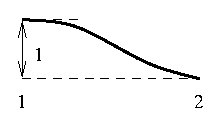
\includegraphics[width=\linewidth]{figs/118curso01}}
\parbox{0.16\textwidth}{$a_1=w_1$}
\\
\parbox{0.46\textwidth}{\[N_2(x)=x\left(1-2\frac{x}{l}+\frac{x^2}{l^2}\right)\]}
\parbox{0.34\textwidth}{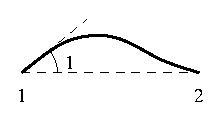
\includegraphics[width=\linewidth]{figs/118curso02}}
\parbox{0.16\textwidth}{$a_2=\left.\frac{\dr w}{\dr x}\right|_1$}
\\
\parbox{0.46\textwidth}{\[N_3(x)=\frac{x^2}{l^2}\left(3-2\frac{x}{l}\right)\]}
\parbox{0.34\textwidth}{\includegraphics[width=\linewidth]{figs/118curso03}}
\parbox{0.16\textwidth}{$a_3=w_2$}
\\
\parbox{0.46\textwidth}{\[N_4(x)=\frac{x^2}{l}\left(\frac{x}{l}-1\right)\]}
\parbox{0.34\textwidth}{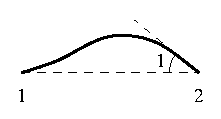
\includegraphics[width=\linewidth]{figs/118curso04}}
\parbox{0.16\textwidth}{$a_4=\left.\frac{\dr w}{\dr x}\right|_2$}
\end{frame}

\begin{frame}
\frametitle{Stiffness Matrix}
%\frametitle{Matriz de rigidez}
Integrating the individual matrix components in \eqref{eq:FMb}
%Integrando términos de (\ref{eq:FMb}):
\begin{gather}
  K_{11}^e=EI\int_0^l B_1^2\,\dr x;
  \quad B_1=\frac{\dr ^2}{\dr x^2}N_1(x)=-\frac{6}{l^2}+\frac{12x}{l^3};
  \\
  K_{11}^e=\frac{12EI}{l^3};
  \\
  K_{12}^e=\frac{6EI}{l^2};
  \quad
  K_{13}^e=-\frac{12EI}{l^3}; \ldots
\end{gather}
\begin{equation}
  \mcolorbox{\displaystyle
  [\mathbf{K}^e]=\frac{12EI}{l^3}
  \begin{pmatrix}
  1 & l/2 & -1 & l/2 \\
  l/2 & l^2/3 & -l/2 & l^2/6 \\
  -1 & -l/2 & 1 & -l/2 \\
  l/2 & l^2/6 & -l/2 & l^2/3
  \end{pmatrix}
  }
\end{equation}
\end{frame}

\begin{frame}
\frametitle{Consistent Load Vectors}
%\frametitle{Matrices de cargas consistentes}
\begin{itemize}
  \item 
  Integrating the individual terms in \eqref{eq:FMb1}, \eqref{eq:FMb} for each element $e$, assuming constant distributed load $q$:
%  Integrando términos de (\ref{eq:FMb1}), (\ref{eq:FMb}) en cada elemento, suponiendo carga $q$ constante:
    \begin{equation}
    \{\mathbf{f}^e\}
  =
    \underbrace{
  \begin{Bmatrix}
  ql/2 \\ ql^2/12 \\ ql/2 \\ -ql^2/12
    \end{Bmatrix}
  }_{\displaystyle \{\mathbf{f}_\text{dist}\}}
    +
  \underbrace{
    \begin{Bmatrix}
    -V_1 \\ -M_1 \\ V_2 \\ M_2
  \end{Bmatrix}
    }_{\displaystyle \{\mathbf{f}_\text{boun}\}}
\end{equation}
\item $\{\mathbf{f}_\text{dist}\}$ 
includes the distributed transverse loads $q$ and the fixed-end moments (\emph{``momentos de empotramiento perfecto''})
%incluye el reparto de las cargas transversales $q$ y los momentos de empotramiento perfecto
\item $\{\mathbf{f}_\text{boun}\}$ 
corresponds to the loads at the ends (boundaries) of the element
%corresponde a los esfuerzos en los extremos del elemento
\end{itemize}
\end{frame}

\begin{frame}
\frametitle{Direct Matrix Formulation (w/o Finite Elements)}
%\frametitle{Formulación matricial directa (sin Elementos Finitos)}
\begin{itemize}
\item
General solution in beam 1--2 without distributed loads $(q=0)$:
%Solución general en tramo 1--2 sin cargas intermedias $(q=0)$:
\parbox[t]{0.3\textwidth}{$\dfrac{\dr ^4w}{\dr x^4}=0$}\hfil
\parbox[c]{0.5\textwidth}{\strut\includegraphics[scale=0.5]{figs/118curso08a}}
\item
Boundary conditions:
%Condiciones de contorno: 
$w_1, \left.\dfrac{\dr w}{\dr x}\right|_1,
w_2, \left.\dfrac{\dr w}{\dr x}\right|_2$
\begin{equation}
  w(x)=\alpha_0+\alpha_1 x+\alpha_2 x^2+\alpha_3 x^3
\end{equation}
4 conditions 
%4 condiciones 
$\quad\Rightarrow\quad 
\text{4 parameters}
%\text{4 parámetros}
\quad (\alpha_0, \alpha_1, \alpha_2, \alpha_3)$\\
\alert{Exact solution with FE interpolation!}
\item
Direct formulation of matrix structural equations
%\emph{Planteamiento directo} de ecuaciones matriciales: programas de <<barras>>
\item
Warning: distributed loads $(q\ne 0)$ require correction (fixed-end moments)
%\alert{Ojo}: cargas repartidas $(q\ne 0)$ precisa corrección (momentos de empotramiento)
\end{itemize}
\end{frame}

\section{Timoshenko Beam}
%\section{Modelo de vigas de Timoshenko}

\subsection{Strong and Weak Formulations}
%\subsection{Formulaciones fuerte y débil}

\begin{frame}
\frametitle{Timoshenko Beam Model: Assumptions}
%\frametitle{Hipótesis de vigas de Timoshenko}
\begin{columns}
\begin{column}{0.4\textwidth}
\begin{enumerate}
  \item 
  Prismatic rod, with base curve \emph{(``directriz'')}  $\bm{r}_{0}(s)$ (line of centroids)
%  Pieza prismática, directriz
  %\newcounter{enumi_saved}
  \setcounter{enumi_saved}{\value{enumi}}
\end{enumerate}
\end{column}
\begin{column}{0.6\textwidth}
  \includegraphics[scale=0.5]{figs/118curso05a}
\end{column}
\end{columns}
\begin{columns}
\begin{column}{0.99\textwidth}
\begin{enumerate}
  \setcounter{enumi}{\value{enumi_saved}}
  \item 
  After deformation, plane cross sections $(yz)$ remain plane but \alert{not necessarily normal to the base curve}  
%  Secciones planas normales a directriz permanecen planas, pero \textcolor{red}{\emph{no necesariamente normales a la directriz.}}
  \item 
  (2D) Displacements normal to the beam $(z)$ are uniform along the cross section and equal to those of the base curve:
%  Desplazamientos normales a la viga son uniformes sobre la sección, e iguales a los de la directriz:
  \begin{equation}
    \boxed{w(x,z)=w(x).} \label{eq:wxzt}
  \end{equation}
  \item 
  (2D) Plane stress:
%  Tensión plana: 
  \begin{equation}
  \boxed{\sigma_{zz}=0.}
  \end{equation}
\end{enumerate}
\end{column}
\begin{column}{0.01\textwidth}
\strut
\end{column}
\end{columns}
\end{frame}

\begin{frame}
\frametitle{Timoshenko Beams: Displacements}
%\frametitle{Vigas de Timoshenko: Desplazamientos}
\begin{itemize}
  \item $\theta$: 
  rotation of cross section;
%  giro sección;
$x$: normal to cross section
  \item $\dr w/\dr x = w'$: 
  rotation of base curve tangent (1st order)
%  giro directriz (1\sptext{er} orden)
\end{itemize}
%\parbox{0.48\textwidth}{
\begin{columns}
\begin{column}{0.45\textwidth}
\includegraphics[width=1.0\linewidth]{figs/118curso09a}
%}
\end{column}
\begin{column}{0.55\textwidth}
\begin{itemize}
%\item[\carreau]
%Rotation of cross section:
%%Giro de sección: 
%$\theta$ \\
%\item[\carreau]
%Rotation of tangent to base curve:
%%Giro de directriz: 
%$\dfrac{\dr w}{\dr x}=w'$\\[1ex]
\item%[\carreau]
Cross section not normal to base curve:
%Sección normal a directriz:
\begin{gather}
  \mcolorbox{\theta\ne\dfrac{\dr w}{\dr x}}
  \label{eq:tnwx}
\end{gather}
\item%[\carreau]
Longitudinal displacements:
%Desplazamiento longitudinal:
\begin{equation}
  u(x,z)=u_0(x)-z\theta
  \label{eq:uxzt}
\end{equation}
\end{itemize}
\end{column}
\end{columns}
\end{frame}

\begin{frame}
\frametitle{Timoshenko Beams: Strains}
%\frametitle{Vigas de Timoshenko: Deformaciones}
From the above displacement equations,
\begin{align}
  \text{(\ref{eq:uxzt}): $\to$} &&\quad
  \varepsilon_{xx}&=\frac{\partial u}{\partial x}
  =\frac{\dr  u_0}{\dr x}-z\frac{\dr \theta}{\dr x}
  \\
  \text{(\ref{eq:wxzt}): $\to$} &&\quad
  \varepsilon_{zz}&=\frac{\partial w}{\partial z}=0;
  \\
  \text{(\ref{eq:uxzt}): $\to$} &&\quad
  \gamma_{xz}&=2\varepsilon_{xz}=\frac{\partial u}{\partial z}+
  \frac{\partial w}{\partial x}=-\theta+\frac{\dr w}{\dr x} \ne 0
  \label{eq:gamma}
  \\
  && \gamma_{yz}&=\gamma_{xy}=0
\end{align}
\begin{block}%
{Implications}
%{Implicaciones}
\begin{itemize}
\item 
\emph{Shear deformation}  $\gamma_{xz}\ne 0$ is considered
%\emph{Sí existe} deformación por cortante $\gamma_{xz}\ne 0$
\item 
Shear deformation is constant across cross section (Navier hypothesis)
%Deformación cortante es constante en sección (hipótesis de Navier)
\item 
Assumption valid for not so slender beams: $\lambda=\dfrac{l}{t}\gtrapprox 8$.
%Hipótesis válida para vigas moderadamente gruesas: $\lambda=\dfrac{l}{t}>8$.
\end{itemize}
\end{block}
\end{frame}

\begin{frame}
\frametitle{Constitutive relations}
%\frametitle{Relaciones Constitutivas}
\begin{itemize}
\item
Stresses
%Tensiones
\begin{align}
  \sigma_{xx}&=E\varepsilon_{xx}=E\frac{\dr  u_0}{\dr x}-Ez\frac{\dr \theta}{\dr x}
  \\
  \sigma_{xz}&=\tau=G\gamma_{xz}=G\left(\frac{\dr w}{\dr x}-\theta\right)
\end{align}
\item
Resultants
%Resultantes
\begin{align}
  M&=\int_{t_{1}}^{t_{2}} -Ez^2\frac{\dr \theta}{\dr x} b(z)\,\dr z
  =EI\frac{\dr \theta}{\dr x}=EI\kappa
  \\
  V&=\int_{t_{1}}^{t_{2}} G\left(\frac{\dr w}{\dr x}-\theta\right) b(z) \,\dr z
  =GA\left(\frac{\dr w}{\dr x}-\theta\right)
  =GA\gamma_{xz}
  \\
  N&=\int_{t_{1}}^{t_{2}} E\left(\frac{\dr  u_0}{\dr x}-z\frac{\dr \theta}{\dr x}\right) b(z)\,\dr z
  =EA\frac{\dr  u_0}{\dr x}
\end{align}
\end{itemize}
\end{frame}

\begin{frame}
\frametitle{Shear: stress distribution in cross section}
%\frametitle{Área Reducida de Cortante}
\begin{itemize}
\item 
Following \eqref{eq:gamma}, shear strain is assumed constant throughout the cross section, which implies a similar constant value for the shear stress
%Según \eqref{eq:gamma}, ,a deformación tangencial es constante a lo largo de la sección, lo que implica un valor igualmente constante para la tensión tangencial
\begin{equation}
	\gamma_{xz}=\gamma_0\ \text{(const.)}
	\quad\Rightarrow\quad
	\tau_{0} = G\gamma_{0} = \frac{V}{A} \ \text{(const.)}
\end{equation}
\item 
However, basic equilibrium requires $\tau=0$ at the top and bottom boundaries.
Assuming for simplicity a rectangular cross section (width $b$, depth $h$), the correct distribution of shear stress $\tau(z)$ consistent with the continuum mechanics equilibrium equations is \alert{parabolic}.
\item
Equating the shear resultant for both cases,
%Igualando el cortante resultante
$V=\int_{A} \tau(z)\,\dr A$:\\
{\centering\includegraphics[scale=0.50]{figs/parabolic-shear-stress}\par}
\item
\emph{Note}: For a parabolic distribution, elasticity equations imply non-uniform shear strain and \alert{warping} of the cross section.
\end{itemize}
\end{frame}

\begin{frame}
\frametitle{Shear: reduced shear area}
%\frametitle{Área Reducida de Cortante}
\begin{itemize} 
\item 
In order to ensure correct shear deformation of the Timoshenko beam model, we now
equate the strain energy for both cases, assuming an \alert{equivalent shear area $A^{*}$}\\
{\centering\includegraphics[scale=0.55]{figs/reduced-shear-area}\par}
%Igualando energía de deformación entre ambos casos, con área reducida $A^{*}$
\begin{equation*}
  \frac{1}{2GA^{*}} V^2 = \frac{1}{2}\int_{A}\frac{1}{G} \tau^{2}(z)\,\dr A
  \quad\Rightarrow\quad A^*=\alpha A.
\end{equation*}
\item 
The \alert{shear correction factor $\alpha$} depends on the shape of the section.
\item
For the \alert{rectangular section}, with $\dr A=b\,\dr z$, the above equation yields
%Sección rectangular:
\begin{equation*}
\mcolorbox{A^*=\dfrac{5}{6} A\ \Rightarrow\  \alpha=\dfrac{5}{6}}
\end{equation*}
\end{itemize}
\end{frame}


\begin{frame}
\frametitle{Strong Formulation}
%\frametitle{Formulación Fuerte}
\begin{itemize}
\item
From equilibrium equations
%A partir de ecuaciones de equilibrio.
\begin{alignat}{3}
  &\text{(\ref{eq:MV}): }\quad
  \frac{\dr M}{\dr x}+V&=0
  &\quad\Rightarrow\quad&
  EI\frac{\dr ^2\theta}{\dr x^2}+V&=0
  \label{eq:FFtM}
  \\
  &\text{(\ref{eq:Vq}): }\quad
  \frac{\dr V}{\dr x}+q&=0
  &\quad\Rightarrow\quad&
  GA^*\left(\frac{\dr ^2w}{\dr x^2}-\frac{\dr \theta}{\dr x}\right)+q&=0
  \label{eq:FFtV}
\end{alignat}
\item 
These include 2nd order derivatives of
%Intervienen derivadas segundas de 
$w, \theta$.
\end{itemize}
\end{frame}

\begin{frame}
\frametitle{Weak Formulation (Moments)}
%\frametitle{Formulación débil (momentos)}
Taking in 1st place the moment equation  (\ref{eq:FFtM}):
%Tomando en primer lugar la ecuación del momento (\ref{eq:FFtM}):
\begin{equation}
  \int_{1}^{2} \bar\theta\,\left(EI\frac{\dr ^2\theta}{\dr x^2}\right)\,\dr x
  + \int_{1}^{2} \bar\theta\,\overbrace{V}^{\displaystyle GA^* \gamma_{xz}}\,\dr x
  =0 \quad\forall{\bar\theta}
\end{equation}
Integrating by parts,
%Integrando por partes,
\begin{multline}
  -\int_1^2 \frac{\dr \bar\theta}{\dr x} EI \frac{\dr \theta}{\dr x}\,\dr x
  +\Bigl[\bar\theta\,EI\frac{\dr \theta}{\dr x} \Bigr]_1^2
  \\
  +\int_1^2 \bar\theta GA^*\left(\frac{\dr w}{\dr x}-\theta\right)\,\dr x
  =0 \quad\forall{\bar\theta}
\label{eq:FDMt}
\end{multline}
\end{frame}

\begin{frame}
\frametitle{Weak Formulation (Shear)}
%\frametitle{Formulación débil (cortantes)}
Doing the same for the shear equation (\ref{eq:FFtV}):
%Haciendo ahora lo mismo con la del cortante (\ref{eq:FFtV}):
\begin{equation}
  \int_{1}^{2}\bar w\,GA^*\left(\frac{\dr ^2w}{\dr x^2}
  -\frac{\dr \theta}{\dr x}\right)\,\dr x
  +\int_{1}^{2} q \bar w\,\dr x
  =0 \quad\forall \bar w
\end{equation}
Integrating by parts:
%Integrando por partes:
\begin{multline}
  -\int_{1}^{2} \frac{\dr \bar w}{\dr x} GA^* \left(\frac{\dr  w}{\dr x}-\theta\right)\,\dr x+
  \Bigl[\bar w\,GA^*\left(\frac{\dr  w}{\dr x}-\theta\right) \Bigr]_1^2
  \\
  +\int_1^2 \bar w q\,\dr x
  =0 \quad\forall \bar w
\label{eq:FDVt}
\end{multline}
\end{frame}

\begin{frame}
\frametitle{Weak Formulation (Joint)}
%\frametitle{Formulación débil (conjunta)}
Adding
%Sumando 
\eqref{eq:FDMt} \& \eqref{eq:FDVt}:
\begin{multline}
  \int_{1}^{2} 
  \underbrace{\left(\frac{\dr \bar w}{\dr x}-\bar\theta\right)}_{\bar\gamma} GA^* 
  \underbrace{\left(\frac{\dr  w}{\dr x}-\theta\right)}_{\gamma}\,\dr x
  +\int_1^2 \underbrace{\frac{\dr \bar\theta}{\dr x}}_{\displaystyle \bar\kappa} 
  EI \underbrace{\frac{\dr \theta}{\dr x}}_{\displaystyle \kappa}\,\dr x
  \\
  =\Biggl[\bar w\, \underbrace{GA^*\left(\frac{\dr  w}{\dr x}-\theta\right)}%
  _{\displaystyle V_i}\Biggr]_1^2
  +\Biggl[\bar\theta\,\underbrace{EI\frac{\dr \theta}{\dr x}}_{\displaystyle M_i}\Biggr]_1^2
  + \int_1^2 \bar w q\,\dr x
  \quad\forall (\bar w,\bar\theta)
  \label{eq:FDt}
\end{multline}
\begin{block}%
{Convergence Requirements}
%{Requisitos para convergencia}
  \begin{itemize}
    \item The weak formulation includes first order derivatives of
%    Intervienen derivadas primeras de 
   $w,\bar w,\theta,\bar\theta$
   \item $\Rightarrow$ 
   FEM requires only  $C^0$ approximation
%   requiere tan solo aproximación $C^0$
\end{itemize}
\end{block}
\end{frame}

\subsection{Finite Element Approximation}
%\subsection{Aproximación de Elementos Finitos}

\begin{frame}
\frametitle{Finite Element Approximation (Galerkin)}
%\frametitle{Aproximación Elementos Finitos (Galerkin)}
\begin{block}{%
Weak formulation (from \eqref{eq:FDt})}
%La formulación débil (\ref{eq:FDt}) puede escribirse:
\begin{multline*}
  \delta W = 
  \int_1^2 \bar\gamma\, GA^* \,\gamma \,\dr x
  +\int_1^2 \bar\kappa\, EI\, \kappa\,\dr x
  -\int_1^2 \bar w\, q\,\dr x
  -\left[\bar w\, V\right]_1^2
  -\left[\bar\theta\, M\right]_1^2
  \\
  =0 \quad\forall(\bar\gamma,\bar\kappa)
\end{multline*}
\end{block}
%\club 
Linear interpolation functions ($C^{0}$ continuity):
%Funciones de interpolación lineales (continuidad $C^0$):
\begin{align*}
  w^h(x)=w_1 N_1(x)+w_2 N_2(x);\\
  \theta^h(x)=\theta_1 N_1(x)+\theta_2 N_2(x);
\end{align*}
\parbox{0.5\textwidth}{\centering\includegraphics[width=0.75\linewidth]{figs/118curso10a}}%
\parbox{0.5\textwidth}{\centering\includegraphics[width=0.75\linewidth]{figs/118curso11a}}
\end{frame}

\begin{frame}
\frametitle{Interpolation of Strains}
%\frametitle{Interpolación de Deformaciones}
\begin{gather*}
  \kappa^h=\theta_1\frac{\dr  N_1}{\dr x}+\theta_2\frac{\dr  N_2}{\dr x}
  =\underbrace{\begin{bmatrix} 0 & -1/l & 0 & 1/l \end{bmatrix}%
  }_{\displaystyle[\mathbf{B}_f^e]}
  \begin{Bmatrix} w_1 \\ \theta_1 \\ w_2 \\ \theta_2 \end{Bmatrix}
  \ \text{(cte.)}
  \\
  \begin{split}
  \gamma^h&=\left(\frac{\dr w^h}{\dr x}-\theta^h\right)
  =w_1\frac{\dr  N_1}{\dr x}-\theta_1 N_1+w_2\frac{\dr  N_2}{\dr x}-\theta_2 N_2
  \\
  &=\underbrace{\begin{bmatrix} -1/l & -1+x/l & 1/l & -x/l \end{bmatrix}%
  }_{\displaystyle[\mathbf{B}_c^e]}
  \begin{Bmatrix} w_1 \\ \theta_1 \\ w_2 \\ \theta_2 \end{Bmatrix}
  \ \text{(linear)}
  \end{split}
\end{gather*}
\end{frame}

\begin{frame}
\frametitle{Element Matrices  (1)}
%\frametitle{Matrices elementales (1)}
\begin{equation*}
  \delta W^{h,e} = \{\bar{\mathbf{a}}^e\}^\text{T} \Biggl[ 
  \Bigl([\mathbf{K}_f^e] + [\mathbf{K}_c^e] \Bigr) \{\mathbf{a}^e\}
  - \{\mathbf{f}_\text{int}^e\} - \{\mathbf{f}_\text{ext}^e\} \Biggr] 
\end{equation*}
\begin{gather*}
  \mcolorbox{\displaystyle
  [\mathbf{K}_f^e]=\int_1^2 [\mathbf{B}_f^e]^\text{T} EI [\mathbf{B}_f^e]\,\dr x\,;
  }
  \qquad
  \mcolorbox{\displaystyle
  [\mathbf{K}_c^e]=\int_1^2 [\mathbf{B}_c^e]^\text{T} GA^* [\mathbf{B}_c^e]\,\dr x
  }
  \\
  \{\mathbf{f}_\text{dist}^e\} = \int_1^2 \{\mathbf{N}^e\} q(x)\,\dr x
  ;\qquad
  \{\mathbf{f}_\text{boun}^e\} = \begin{Bmatrix} -V_1 \\ -M_1 \\ V_2 \\ M_2 \end{Bmatrix}
\end{gather*}
\end{frame}

\begin{frame}
\frametitle{Element Matrices (2)}
%\frametitle{Matrices elementales (2)}
Exact closed form integration:
%Integrando analíticamente:
\begin{align*}
  [\mathbf{K}_f^e] &= \left(\frac{EI}{l}\right)^e
  \begin{pmatrix}
  0 & 0 & 0 & 0 \\
  0 & 1 & 0 & -1 \\
  0 & 0 & 0 & 0 \\
  0 & -1 & 0 & 1
  \end{pmatrix}
  \quad&&\text{\parbox{19ex}%
  {\flushleft (constant: 1 Gauss point)}}
%  {(constante: 1 pto. Gauss)}}
  \\
  [\mathbf{K}_c^e] &= \left(\frac{GA^*}{l}\right)^e
  \begin{pmatrix}
  1 & l/2 & -1 & l/2 \\
  l/2 & l^2/3 & -l/2 & l^2/6 \\
  -1 & -l/2 & 1 & -l/2 \\
  l/2 & l^2/6 & -l/2 & l^2/3
  \end{pmatrix}
  \quad&&\text{\parbox{19ex}%
  {\flushleft (quadratic: 2 Gauss points)}}
%  {(cuadrático: 2 ptos. Gauss)}}
\end{align*}
\end{frame}

\section{Performance of beam models}
%\section{Locking in Slender Beams}
%\section{Problemas de bloqueo en vigas esbeltas}

\subsection{Comparison of models}

\begin{frame}
\frametitle{Deformation of Cantilever}
%\frametitle{Deformación de ménsula}
\begin{itemize}[<+->]
\item Bernoulli beam
%\club Viga Bernoulli 
$(EI)$: $w_f=P\dfrac{l^3}{3EI}$
\hfill\parbox{0.42\textwidth}{\visible<1->{\includegraphics[scale=0.5]{figs/118curso13a}}\hfill}
\item Shear beam\\
\blue{(idealisation)}
%\club Viga Cortante 
$(GA^*)$: $w_c=P\dfrac{l}{GA^*}$
\hfill\parbox{0.42\textwidth}{\visible<2->{\includegraphics[scale=0.5]{figs/118curso14a}}\hfill}
\item  Timoshenko beam
%\club Viga Timoshenko 
$(EI, GA^*)$:\\
$w_t=P\left(\dfrac{l^3}{3EI}+\dfrac{l}{GA^*} \right)$
\hfill\parbox{0.42\textwidth}{\visible<.->{\includegraphics[scale=0.5]{figs/118curso15a}}\hfill}\\
(\alert{more flexible than Bernoulli !})
%(Más flexible que viga Bernoulli)
\end{itemize}
\end{frame}

\begin{frame}
\frametitle{\insertsubsection{} -- Shear deflection}
\begin{itemize}[<+->]
\item[\club]
Assuming rectangular cross section
%Sección rectangular 
\begin{equation*}
  I=\frac{1}{12}bt^3;\qquad A^*=\frac{5}{6} bt
\end{equation*}
\item[\club]
The bending and shear stiffness coefficients are:
\begin{equation*}
  K_f=\frac{3EI}{l^3};\qquad
  K_c=\frac{GA^*}{l}
\end{equation*}
\item[\club]
The ratio $K_{f}/K_{c}$ gives the relative value of shear deflection over bending deflection; it quantifies the relevance of Timoshenko beam:
\begin{equation*}
  \frac{K_f}{K_c}=\frac{3}{5}(1+\nu)\frac{1}{\lambda^2}
  \qquad (\lambda=\frac{l}{t}\,,\text{ slenderness})
\end{equation*}
\item[\club]
Example: assuming $\nu=0.25$,\qquad
\begin{tabular}{c|c}
$\lambda$ & $K_{f}/K_{c}$ \\
\hline\hline
$10$ & $0.75\,\%$\\
$3$ & $8.33\,\%$
\end{tabular}
\end{itemize}
\end{frame}

\begin{frame}
\frametitle{Example of cantilever beam FE models}
\begin{columns}
\begin{column}{0.5\textwidth}
\centering
\includegraphics[width=\linewidth]{figs-abaqus/empb10-u2.pdf}\\
\includegraphics[width=\linewidth]{figs-abaqus/empt10-u2.pdf}\\
$
\lambda=\dfrac{l}{t}=10\ \Rightarrow\ \dfrac{u_{t}-u_{b}}{u_{b}}=0.68\,\%
$\\
\Green{acceptable error}
\end{column}
\begin{column}{0.5\textwidth}
\centering
\includegraphics[width=\linewidth]{figs-abaqus/empb3-u2.pdf}\\
\includegraphics[width=\linewidth]{figs-abaqus/empt3-u2.pdf}\\
$
\lambda=\dfrac{l}{t}=3\ \Rightarrow\ \dfrac{u_{t}-u_{b}}{u_{b}}=8.08\,\%
$\\
\alert{excessive error!}
\end{column}
\end{columns}
\end{frame}

\subsection{Locking and solutions}

\begin{frame}
\frametitle{Locking of (Timoshenko) Slender Beam}
\begin{itemize}[<+->]
\item
In principle, it would be desirable to use the more general Timoshenko model for all cases, including slender beams.
\item
In the limit for very slender beams:
\begin{equation*}
  \lambda\rightarrow\infty
  \quad\Rightarrow\quad
  \frac{K_f}{K_c}\rightarrow 0,
  \ \theta=\frac{\dr w}{\dr x}
\end{equation*}
\item
Considering the FE approximation in a cantilever, with linear interpolation functions for $w$ and $\theta$ around node 1
\centerline{\visible<3->{\includegraphics[scale=0.6]{figs/118curso16a}}}
\item
Starting from the fixed end, the interpolation implies the propagation to the adjoining nodes:
\end{itemize}
\uncover<4->{%
$\theta_0=0 \ \Rightarrow\ \left.\dfrac{\dr w}{\dr x}\right|_0=0
\stackrel{\text{($w$ linear in elem.)}}{\Rightarrow}
%\text{($w$ lineal en elto.)}
\ w_1=0,\ \theta_1=0\ \Rightarrow\ \left.\dfrac{\dr w}{\dr x}\right|_1=0,
\ldots$
\\
\centerline{\fbox{\color{red}locking!}}
%\fbox{\color{red}¡Bloqueo!}
}
\end{frame}

\begin{frame}
\frametitle{Example: Cantilever with 1 element (1)}
%\frametitle{Ejemplo: ménsula con 1 elemento (1)}
\club
\parbox{0.6\textwidth}%
{1 element Timoshenko beam}
%{1 elemento viga de Timoshenko}
\hfill
\parbox{0.35\textwidth}{\hfill\includegraphics[scale=0.5]{figs/118curso17a}}
\begin{equation*}
  \begin{pmatrix}
  \frac{GA^*}{l} & \frac{GA^*}{2} & -\frac{GA^*}{l} & \frac{GA^*}{2} \\
                 & \frac{GA^*}{3}l+\frac{EI}{l} & -\frac{GA^*}{2} & 
		 \frac{GA^*}{6}l-\frac{EI}{l} \\
                 & & \frac{GA^*}{l} & -\frac{GA^*}{2} \\
		 & & & \frac{GA^*}{3}l+\frac{EI}{l}
  \end{pmatrix}
  \begin{Bmatrix} 0 \\ 0 \\ w_2 \\ \theta_2 \end{Bmatrix}
  =
  \begin{Bmatrix} V_1 \\ M_1 \\ P \\ 0 \end{Bmatrix}
\end{equation*}
\club
Eliminating the equations for 
%Eliminando las ecuaciones de
$(V_1, M_1)$:
\begin{equation*}
  \begin{pmatrix}
  \frac{GA^*}{l} & -\frac{GA^*}{2} \\
  -\frac{GA^*}{2} & \frac{GA^*}{3}l+\frac{EI}{l}
  \end{pmatrix}
  \begin{Bmatrix} w_2 \\ \theta_2 \end{Bmatrix}
  =
  \begin{Bmatrix} P \\ 0 \end{Bmatrix}
\end{equation*}
\end{frame}

\begin{frame}
\frametitle{Example: Cantilever with 1 element (2)}
%\frametitle{Ejemplo: ménsula con 1 elemento (2)}
\club 
Inverting:
%Invirtiendo:
\begin{gather*}
  \begin{Bmatrix} w_2 \\ \theta_2 \end{Bmatrix}
  =
  \text{\color{blue}$\dfrac{\mu}{1+\mu}$}
  \begin{pmatrix}
  \frac{l}{GA^*}+\frac{l^3}{3EI} & \frac{l^2}{2EI} \\
  \frac{l^2}{2EI} & \frac{l}{2EI}
  \end{pmatrix}
  \begin{Bmatrix} P \\ 0 \end{Bmatrix}
  \quad
  \left(\mu=\frac{12EI}{GA^* l^2}\right)
  \\
  w_2 = \dfrac{\mu}{1+\mu} P \left(\frac{l}{GA^*}+\frac{l^3}{3EI}\right)
\end{gather*}
\club 
Identical to exact solution (with bending and shear),\\
 except for the factor
%Idéntica a solución exacta (con flexión y cortante), salvo el factor
\mcolorbox{\dfrac{\mu}{1+\mu}}. 

\club 
Value for an infinitely slender rectangular section beam
%Valor para sección rectangular 
$(b\times t)$ \& $\nu=1/4$:
\begin{equation*}
  \frac{\mu}{1+\mu}=\frac{3}{3+\lambda^2};
  \quad
  \lim_{\lambda\rightarrow\infty}\frac{\mu}{1+\mu}=0
  \ \Rightarrow\ \mcolorbox{w_{2}=0}
\end{equation*}
\centerline{\fbox{\color{red} Locking!}}
%\centerline{\fbox{\color{red} ¡Bloqueo!}}
\end{frame}

%\subsection{Solutions}

\begin{frame}
\frametitle{Reduced Integration}
%\frametitle{Integración reducida}
\begin{itemize}
  \item 
  In principle it would be necessary to integrate at one point the bending terms and at two points the shear terms
%  En principio sería necesario integrar en un punto los términos de flexión y en dos puntos los de cortante.
  \item 
  It is possible to modify these integration rules so as to relax the locking exhibited by these elements
%  Es posible modificar estas reglas de integración para relajar el bloqueo que exhiben estos elementos.
  \item 
  Particularising  $[\mathbf{K}_c]$ at the center of the element, and integrating with only one point:
%  Particularizando $[\mathbf{K}_c]$ en el centro del elemento, e integrando con este único punto de integración: 
\begin{equation*}
\begin{split}
  [\mathbf{K}_c^e]
  &=\int_1^2 \Bigl[\mathbf{B}_c^e\Bigr]_{x=l/2}^\text{T} 
  GA^* \Bigl[\mathbf{B}_c^e\Bigr]_{x=l/2}\,\dr x
  \\
  &= \left(\frac{GA^*}{l}\right)^e
  \begin{pmatrix}
  1 & l/2 & -1 & l/2 \\
  l/2 & l^2/4 & -l/2 & l^2/4 \\
  -1 & -l/2 & 1 & -l/2 \\
  l/2 & l^2/4 & -l/2 & l^2/4
  \end{pmatrix}
\end{split}
\end{equation*}
\end{itemize}
\end{frame}

\begin{frame}
\frametitle{Cantilever, 1 element Reduced Integration}
%\frametitle{Ménsula, 1 elto. de integración reducida}
\begin{itemize}[<+->]
\item[\club] 
Matrix equation:
%Ecuación matricial:
\begin{equation*}
  \begin{Bmatrix} w_2 \\ \theta_2 \end{Bmatrix}
  =
  \begin{pmatrix}
  \frac{l}{GA^*}+\frac{l^3}{\text{\textcolor{blue}{$4$}}%
  EI} & \frac{l^2}{2EI} \\
  \frac{l^2}{2EI} & \frac{l}{2EI}
  \end{pmatrix}
  \begin{Bmatrix} P \\ 0 \end{Bmatrix}
\end{equation*}
\item[\club] 
For
%Para 
$\lambda\rightarrow\infty$:
\begin{equation*}
  \frac{w^\text{FE}}{w^\text{exact}}
  \to
  \frac{l^3/(4EI)}{l^3/(3EI)}=\frac{3}{4} 
\end{equation*}
\alert{Locking-free solution!} \\
(although slightly  stiffer than exact solution)
%¡Solución sin bloqueo!  (algo más rígido que solución exacta)
\item[\club] 
The error vanishes for a sufficiently refined mesh:\\
%El error desaparece para una malla suficientemente fina:
with only 2 elements, 
%con tan sólo 2 elementos, 
$w^\text{FE}/w^\text{exact}=0.938$ 
(for
%(para
$\lambda\rightarrow\infty$).
\end{itemize}
\end{frame}

\begin{frame}
\frametitle{Assumed Strains (1)}
%\frametitle{Deformaciones impuestas (1)}
\bul 
Strain field (Timoshenko, linear interpolation):
%Campo de deformaciones (Timoshenko, interpolación lineal):
\begin{equation*}
  \gamma=\frac{1}{l}(w_2-w_1)+\theta_1\left(1-\frac{x}{l}\right)
  +\theta_2\left(-\frac{x}{l}\right)
\end{equation*}
\bul 
Using isoparametric coordinates:
%En coordenadas isoparamétricas:
\parbox{40mm}{\small \includegraphics[scale=0.5]{figs/118curso18a} }
\begin{equation*}
  \gamma=\underbrace{\frac{1}{l}(w_2-w_1)-\frac{1}{2}(\theta_1+\theta_2)}%
  _{\displaystyle\alpha_1}+
  \underbrace{\frac{1}{2}(\theta_1-\theta_2)}_{\displaystyle\alpha_2}\xi
  =\alpha_1+\alpha_2\xi
\end{equation*}
\bul 
Very slender beams:
%Vigas muy esbeltas: 
\[\alpha_1\rightarrow 0\ \Rightarrow\
\alpha_2\rightarrow 0\ \Rightarrow\ \theta_1=\theta_2\]
\club 
Solution: independent (\alert{``assumed''}) field,
%Solución: campo independiente (\textcolor{red}{<<impuesto>>}),
$\gamma(x)=[\mathbf{N}_{\gamma}]\{\bm{\gamma}\}$
\end{frame}

\begin{frame}
\frametitle{Assumed Strains (2)}
%\frametitle{Deformaciones impuestas (2)}
\begin{itemize}[<+->]
\item
\alert{Mixed method}: independent interpolation of deflections $(w)$, rotations $(\theta)$ and shear strains $(\gamma)$
%\alert{Método \emph{mixto}}: interpolación independiente de flechas $(w)$, giros $(\theta)$, y deformaciones a cortante $(\gamma)$
\item
Simplest case: prescribe
%Caso más simple: imponer 
$\gamma=\text{const.}$:
\begin{equation*}
\begin{split}
  \gamma(\xi)&=[\widehat{\mathbf{B}}_c]\{\mathbf{a}\}
  =\alpha_1=\frac{1}{l}(w_2-w_1)-\frac{1}{2}(\theta_1+\theta_2)
  \\
  &=\begin{bmatrix} -\frac{1}{l} & -\frac{1}{2} & \frac{1}{l} & -\frac{1}{2}
  \end{bmatrix} 
  \begin{Bmatrix} w_1 \\ \theta_1 \\ w_2 \\ \theta_2 \end{Bmatrix} 
\end{split}
\end{equation*}
\item
In this case, identical result to reduced integration
%En este caso, igual resultado que integración reducida.
\end{itemize}
\end{frame}

\subsection{Continuum elements?}

\begin{frame}
\frametitle{\insertsubsection{} -- 1}
\begin{columns}
\begin{column}{0.4\textwidth}
\begin{block}{Remarks}
%\begin{block}{Objetivos}
\begin{itemize}[<+->]
	\item
	A bilinear continuum element when subjected to \alert{pure bending} is constrained to deform by shear and behaves as too stiff. The solution may be very poor and requires very fine meshes for an acceptable precision.
%	Un elemento bilineal de continuo sometido a \alert{flexión} pura se ve obligado a deformarse por cortante y resulta demasiado rígido. La solución puede ser muy pobre y requerir mallas muy finas para una precisión decente.
	\item
	The \alert{``incompatible modes''} allow a dramatic improvement
%	Los \alert{``modos incompatibles''} permiten mejorar la respuesta en elementos lineales. 
	\item
	\alert{Quadratic} elements also improve results, with additional dof's
%	Los elementos cuadráticos también mejoran este problema, con más gdl.
\end{itemize}
\end{block}
\end{column}
\begin{column}{0.6\textwidth}
\visible<1->{%
ABAQUS Continuum Plane Strain (CPS):\\
CPS4: bilinear; 
\visible<3->{\Green{CPS8}: quadratic;}\\
\visible<2->{\blue{CPS4I}: incompatible modes;}\\
\visible<4->{\red{CPS4R}: reduced integration}
%\includegraphics[width=0.65\linewidth]{figs3/incompatible-modes-2}%
}\\
\centering
\includegraphics[width=0.6\linewidth]{figs4/cps4i-r.png}%
\parbox[b]{0.45\linewidth}{\small 
CPS4: $u=2.25$\\
\visible<2->{\blue{CPS4I: $u=3.04$}}\\
\visible<4->{\red{CPS4R: $u=1207$}}}
\\[2ex]
\includegraphics[width=0.6\linewidth]{figs4/cps4x5r.png}%
\parbox[b]{0.4\linewidth}{\small 
CPS4: $u=3.00$\\
\visible<2->{\blue{CPS4I: $u=3.06$}}\\
\visible<3->{\Green{CPS8: $u=3.06$}}}
\\[2ex]
\visible<3->{%
\includegraphics[width=0.6\linewidth]{figs4/cps8.png}%
\parbox[b]{0.4\linewidth}{\small 
\visible<3->{\Green{CPS8: $u=3.05$}}}}
\end{column}
\end{columns}
\end{frame}

\begin{frame}
\frametitle{\insertsubsection{} -- 2}
Consider a bilinear quad, under pure bending $\to$ prescribed displacement field $\bar{u}$ (extension in top fibre and compression in bottom fibre):
%Se considera un cuadrilátero bilineal, sometido a flexión pura, mediante una deformación impuesta $\bar{u}$ (extensión en la fibra superior y compresión en la inferior):
\begin{columns}
\begin{column}{0.33\textwidth}
\centering
\visible<1->{%
\includegraphics[width=\linewidth]{figs3/incompatible-modes-1}\\
\emph{Bilinear parent element}
%Elemento patrón bilineal
}
\end{column}
\begin{column}{0.33\textwidth}
\centering
\visible<2->{%
\includegraphics[width=\linewidth]{figs3/incompatible-modes-2}\\
\emph{Bilinear quad, required bending moment \Green{$M_{1}$}.}
%Cuadrilátero bilineal, momento flector necesario $M_{1}$.
}
\end{column}
\begin{column}{0.33\textwidth}
\centering
\visible<3->{%
\includegraphics[width=\linewidth]{figs3/incompatible-modes-3}\\
\emph{Elastic solid, required bending moment \Green{$M_{2}$}.}
%Sólido elástico, momento flector necesario $M_{2}$.
}
\end{column}
\end{columns}
\vspace{1ex}
\uncover<4->{
The constraints imposed by the shape functions for the bilinear quad require a greater applied moment than the real one (elastic solid):\\
%Las restricciones que imponen las funciones de interpolación exigen un momento aplicado mayor que el real:
\begin{equation*}
	\mcolorbox{M_{1}>M_{2}}
\end{equation*}
}
\end{frame}

\section{ABAQUS beam models}

\subsection{2D beams}

\begin{frame}
\frametitle{Part definition (1)}
\centering
\includegraphics[scale=0.45]{figs-abaqus/00_create-part-0.png}
\end{frame}

\begin{frame}
\frametitle{Part module (2)}
\centering
\includegraphics[scale=0.30]{figs-abaqus/00_create-part-1.png}
\end{frame}

\begin{frame}
\frametitle{Property module}
\begin{columns}
\begin{column}{0.35\textwidth}
\includegraphics[scale=0.38]{figs-abaqus/01_create-section-1.png}
\end{column}
\begin{column}{0.65\textwidth}
\includegraphics[scale=0.38]{figs-abaqus/01_create-section-2-before.png}
\end{column}
\end{columns}
\end{frame}

%\begin{frame}
%\frametitle{Property module}
%\includegraphics[scale=0.35]{figs-abaqus/01_create-section-shear.png}
%\end{frame}

\begin{frame}
\frametitle{Property module -- beam section}
\begin{columns}
\begin{column}{0.40\textwidth}
\includegraphics[scale=0.35]{figs-abaqus/01_create-section-profile.png}
\end{column}
\begin{column}{0.60\textwidth}
\includegraphics[scale=0.28]{figs-abaqus/02_assign-orient-4.png}
\end{column}
\end{columns}
\end{frame}

\begin{frame}
\frametitle{Property module -- profile and orientation}
\centering
\includegraphics[scale=0.33]{figs-abaqus/03-view-part0.png}
\end{frame}

\begin{frame}
\frametitle{Property module -- display options}
\centering
\includegraphics[scale=0.33]{figs-abaqus/03-view-part1.png}
\end{frame}

\begin{frame}
\frametitle{Load module -- line load}
\centering
\includegraphics[scale=0.40]{figs-abaqus/05_line-load-1.png}\\[2ex]
\includegraphics[scale=0.40]{figs-abaqus/05_line-load-2.png}
\end{frame}

\begin{frame}
\frametitle{Mesh module -- seeds}
\centering
\includegraphics[scale=0.40]{figs-abaqus/06_0_mesh-seeds1.png}
\end{frame}

\begin{frame}
\frametitle{Mesh module -- beam element type}
\begin{columns}
\begin{column}{0.60\textwidth}
\includegraphics[scale=0.30]{figs-abaqus/06_element-type0.png}
\end{column}
\begin{column}{0.40\textwidth}
\includegraphics[scale=0.23]{figs-abaqus/07_element-eb.png}
\includegraphics[scale=0.23]{figs-abaqus/07_element-timo.png}
\end{column}
\end{columns}
\end{frame}

\begin{frame}
\frametitle{Results}
\centering
\includegraphics[scale=0.30]{figs-abaqus/07_results-1.png}
\end{frame}

\begin{frame}
\frametitle{Results}
\centering
\includegraphics[scale=0.30]{figs-abaqus/07_results-3.png}
\end{frame}

\begin{frame}
\frametitle{Results}
\centering
\includegraphics[scale=0.30]{figs-abaqus/07_results-4.png}
\end{frame}

\begin{frame}
\frametitle{Results}
\centering
\includegraphics[scale=0.30]{figs-abaqus/07_results-5.png}
\end{frame}

\end{document}

\section{FEAP commands}

\subsection{2D frame elements}

\begin{frame}[fragile=singleslide]
\frametitle{2D beam without shear deformation (E-B)}
\begin{exampleblock}%
{2D frame element}
\begin{verbatim}
parameter
 t=2.0                       ! Canto de la seccion
 b=1.0                       ! Base de la seccion
 I=(1/12.)*b*t^3             ! Inercia de la viga
 A=b*t                       ! Area de la seccion
 E=3.0e10                    ! Modulo elastico
 nu=0.3                      ! Modulo de Poisson

mate,1
 frame
 shear,off
 cross,section,A,I           ! A, Ixx
 elastic,isotropic,E,nu

\end{verbatim}
\end{exampleblock}
\end{frame}

\begin{frame}[fragile=singleslide]
\frametitle{2D beam with shear deformation (T)}
\begin{exampleblock}%
{2D frame element}
\begin{verbatim}
parameter
 t=2.0                       ! Canto de la seccion
 b=1.0                       ! Base de la seccion
 I=(1/12.)*b*t^3             ! Inercia de la viga
 A=b*t                       ! Area de la seccion
 E=3.0e10                    ! Modulo elastico
 nu=0.3                      ! Modulo de Poisson

mate,1
 frame
 shear,on
 cross,section,A,I,,,,5/6    ! A, Ixx, , , , kx
 elastic,isotropic,E,nu

\end{verbatim}
\end{exampleblock}
\end{frame}

\begin{frame}[fragile=singleslide]
\frametitle{2D beam with shear deformation, enhanced}
\begin{exampleblock}%
{2D frame element}
\begin{verbatim}
parameter
 t=2.0                       ! Canto de la seccion
 b=1.0                       ! Base de la seccion
 I=(1/12.)*b*t^3             ! Inercia de la viga
 A=b*t                       ! Area de la seccion
 E=3.0e10                    ! Modulo elastico
 nu=0.3                      ! Modulo de Poisson

mate,1
 frame
 shear,on
 enhance
 cross,section,A,I,,,,5/6    ! A, Ixx, , , , kx
 elastic,isotropic,E,nu

\end{verbatim}
\end{exampleblock}
\end{frame}


\subsection{3D frame elements}

\begin{frame}
\frametitle{3D beams: Orientation of Cross Section}
\begin{itemize}
\item
For 3D beams it is necessary to define the orientation of the cross section in space
\item
This is determined by the local axes with unit vectors $(\bm{t}_{1}, \bm{t}_{2})$, normal to the axial direction $\bm{t}_{3}$ in the reference configuration
\item
In FEAP, the user must define a \emph{reference vector} $\bm{v}$ which together with $\bm{t}_{3}$ defines the local triad as follows
\end{itemize}
\begin{columns}
\begin{column}{0.6\textwidth}
\begin{block}{Reference vector $\bm{v}$ (manual, p53)}
\begin{itemize}
\item
$\bm{t}_{3}$ axial, longitudinal direction of beam
\item
$\bm{T}_{1}=\bm{v}\times\bm{t}_{3}\,;\quad \bm{t}_{1}=\bm{T}_{1}/|\bm{T}_{1}|$
\item
$\bm{t}_{2} = \bm{t}_{3}\times\bm{t}_{1}$
\item may alternatively use a point, or a node
\end{itemize}
\end{block}
\end{column}
\begin{column}{0.4\textwidth}
\includegraphics[width=\linewidth]{figs/refevect}
\end{column}
\end{columns}
\end{frame}

\begin{frame}[fragile=singleslide]
\frametitle{3D beam with shear deformation}
\begin{exampleblock}%
{3D frame element}
\begin{verbatim}
parameter
 a  = 0.15*0.025+0.125+0.025
 i1 = 2024.44e-8
 i2 = 852.07e-8
 xy = 721.22e-8 * 1e-4
 j  = 140e-8

material 1
 frame
 small
 shear on
 elastic isotropic 2.1e11 0.3
 cross section a i1 i2 xy j 5/6 5/6
 reference vector 0.0 0.0 1.0

\end{verbatim}
\end{exampleblock}
\end{frame}


\appendix
\section*{Bibliography}
%\section{Bibliografía}

\begin{frame}
\frametitle{\insertsection}
%\begin{itemize}%[label=\protect\pica]
\setbeamertemplate{bibliography item}[book]
\begin{thebibliography}{99}
  \bibitem{Onate2013} Eugenio Oñate,
  \newblock\emph{Structural Analysis with the Finite Element Method, Linear Statics; Vol 2: Beams, Plates and Shells},
  CIMNE--Springer, 2013.
  \bibitem{Onate1995} Eugenio Oñate,
  \newblock\emph{Cálculo de Estructuras por el Método de Elementos Finitos},
  Centro Internacional de Métodos Numéricos en Ingeniería, 1995.
  \bibitem{Ottosen-Peterson} N. Ottosen and H. Petersson,
  \newblock\emph{Introduction to the Finite Element Method}, Prentice Hall Europe,
  1992.
  \bibitem{Hughes} Thomas J.R. Hughes,
  \newblock\emph{The Finite Element Method}, Prentice Hall, 1987. 
% \item Michel Géradin y Alberto Cardona,\\
% \emph{Flexible Multibody Dynamics, A Finite Element Approach},
% Wiley, 2001
%\end{itemize}
\end{thebibliography}
\end{frame}

\end{document}
